\documentclass[12pt]{book}

\title{Analysis II}
\author{Fall Semester\\MATH201}
\date{}
\usepackage{indentfirst}
\usepackage{kotex}
\usepackage{amsmath, amssymb, amsthm, amsfonts, graphics, epsfig, fancyhdr, bm, setspace, graphicx}
\usepackage[shortlabels]{enumitem}
\setlength{\headheight}{28pt}
\pagestyle{fancy}
\fancyhf{}
\fancyhead[R]{Ch5. Differentiation}
\fancyfoot[C]{\thepage}

\setlength\parindent{12pt}
\theoremstyle{definition}
\newtheorem{theorem}{Theorem}
\newtheorem{lemma}{Lemma}
\newtheorem{corollary}[theorem]{Corollary}
\newtheorem{proposition}[theorem]{Proposition}
\newtheorem{remark}[theorem]{Remarks}
\newtheorem{definition}[theorem]{Definition}
\newtheorem{example}{Example}
\newtheorem{exercise}{Exercise}

\usepackage{chngcntr}
% \counterwithin{theorem}{chapter}
\counterwithin{exercise}{chapter}
\counterwithin{example}{chapter}
\counterwithin{equation}{exercise}

\setcounter{chapter}{4}
\allowdisplaybreaks
\renewcommand{\theequation}{\arabic{equation}}
\renewcommand{\qedsymbol}{}
\newcommand{\N}{\mathbb{N}}
\newcommand{\Z}{\mathbb{Z}}
\newcommand{\Q}{\mathbb{Q}}
\newcommand{\R}{\mathbb{R}}
\newcommand{\C}{\mathbb{C}}
\newcommand\cdotfill{%
	\leavevmode\cleaders\hb@xt@.44em{\hss$\cdot$\hss}\hfill\kern\z@
}
\makeatletter
\newcommand{\chapterauthor}[1]{%
  {\parindent0pt\vspace*{-25pt}%
  \linespread{1.1}\large\scshape#1%
  \par\nobreak\vspace*{35pt}}
  \@afterheading%
}
\newcommand{\chapterother}[1]{%
  {\parindent0pt\vspace*{-25pt}%
  \linespread{1.1}#1%
  \par\nobreak\vspace*{35pt}}
  \@afterheading%
}
\makeatother

\begin{document}
	\chapter{Differentation\\Selected Exercise homework}
	\chapterauthor{Sung Jae Hyuk}
	\chapterother{Junior in Korea university\\ Majoring in computer science \& mathematics\\Email: okaybody10@korea.ac.kr}
	\newpage
	\begin{exercise}
		Let $f$ be defined for all real $x$, and suppose that
		\begin{equation*}
			|f(x)-f(y)|\leq (x-y)^2
		\end{equation*}
		for all real $x$ and $y$. Prove that $f$ is constant.
	\end{exercise}
	\begin{proof}
		Let $x$, $y$ be real number with $x\neq y$.\\
		As $|x-y|>0$,
		\begin{equation*}
			|f(x)-f(y)|\leq(x-y)^2\\
			\Rightarrow \left\vert \dfrac{f(x)-f(y)}{x-y}\right\vert\leq |x-y|
		\end{equation*}
		By squeeze theorem, $\displaystyle\lim_{x\rightarrow y} \dfrac{f(x)-f(y)}{x-y}$ exists, and that is $0$.\\
		By definition of differentinate, $f'(y)=0$ for all $y\in\R$.\\
		Hence \textbf{Theorem 5.9(c)}, $f(y)$ is constant function for $y\in\R$.
	\end{proof}
	\newpage
	\begin{exercise}
		Suppose $f\,'(x)>0$ in $(a,\,b)$. Prove that $f$ is strictly increasing in $(a,\,b)$, and let $g$ be its inverse function. Prove that $g$ is differentiable, and that
		\begin{equation*}
			g\,'(f(x))=\dfrac{1}{f\,'(x)}\qquad (a<x<b).
		\end{equation*}
	\end{exercise}
	\begin{proof}
		As $f'(x)>0$ in $(a,\,b)$, then $f$ is monotonically increasing function, $i.e.~f$ is one-to-one corresponding.\\
		So we can assume that $g$ is also not only one-to-one but continuous in $(f(a),\,f(b))$\\
		Let $c$ be real number in $(f(a),\,f(b))$.\\
		By definition of continuous, $\displaystyle\lim_{x\rightarrow c} g(x)=g(c)$.\\
		More Specifically, there exists unique $x^*$, $a^*$ in $(a,\,b)$ such that $f(x^*)=x$, $g(c^*)=c$, and
		\begin{equation}
			\displaystyle\lim_{x\rightarrow c} x^*=c^*
		\end{equation}
		Also, $\dfrac{1}{f'(c^*)}$ is well-defined since $f'(c^*)>0$, so
		\begin{equation}
			\displaystyle\lim_{x^*\rightarrow c^*}\dfrac{1}{\dfrac{f(x^*)-f(c^*)}{x^*-c^*}}=\dfrac{1}{f'(c^*)}
		\end{equation}
		Let $\varepsilon>0$.\\
		There exists $\delta_1>0$ such that $\left\vert\dfrac{1}{\dfrac{f(x^*)-f(c^*)}{x^*-c^*}}-\dfrac{1}{f(c^*)}\right\vert<\varepsilon$ for $|x^*-c^*|<\delta_1$ at (2).\\
		Also, there exists $\delta_2>0$ such that $|x^*-c^*|<\delta_1$ for $|x-c|<\delta_2$ at (1).\\
		Since $f(x^*)=x$ and $f(c^*)=c$, $g(x)=x^*$ and $g(c)=c^*$\\
		By above formulas, there exists $\delta_2>0$ such that $\left\vert\dfrac{g(x)-g(c)}{x-c}-\dfrac{1}{f'(c^*)}\right\vert<\varepsilon$ for $|x-c|<\delta_2$.\\
		By definition, $\displaystyle\lim_{x\rightarrow c}\dfrac{g(x)-g(c)}{x-c}=g'(c)$, so $g'(c)=g'(f(c^*))=\dfrac{1}{f'(c^*)}$ for all $c^*\in (a,\,b)$, and proof is completed.
	\end{proof}
	\newpage
	\begin{exercise}
		Suppose $g$ is a real function on $\R$, with bounded derivative (say $|g'|\leq M$). Fix $\varepsilon >0$, and define $f(x)=x+\varepsilon g(x)$. Prove that $f$ is one-to-one if $\varepsilon$ is small enough.\\
		(A set of admissible values of $\varepsilon$ can be determined which depends only on $M$.)
	\end{exercise}
	\begin{proof}
		Since $x$, $g(x)$ are differentiable on $\R$, $f(x)=x+\varepsilon g(x)$ is also differentiable on $\R$ by \textbf{Theorem 5.3}.\\
		Let $0<\varepsilon<\dfrac{1}{2M}$.\\
		\begin{align*}
			f'(x)=1+\varepsilon g'(x) &\geq 1-\varepsilon |g'(x)|\\
			&\geq 1-\varepsilon M\\
			&>1-\dfrac{1}{2M}\cdot M=1-\dfrac{1}{2}=\dfrac{1}{2}
		\end{align*}
		Thus $f'(x)\geq\dfrac{1}{2}>0$, $f(x)$ is monotonically increasing function, one-to-one.
	\end{proof}
	\newpage
	\begin{exercise}
		If
		\begin{equation*}
			C_0+\dfrac{C_1}{2}+\cdots+\dfrac{C_{n-1}}{n}+\dfrac{C_n}{n+1}=0,
		\end{equation*}
		where $C_0,...,\ C_n$ are real constants, prove that the equation
		\begin{equation*}
			C_0+C_1x+\cdots+C_{n-1}x^{n-1}+C_nx^n=0
		\end{equation*}
		has at least one real root between $0$ and $1$.
	\end{exercise}
	\begin{proof}
		Define function $g$ by
		\begin{equation*}
			g(x)=\displaystyle\sum_{i=1}^{n+1}\dfrac{C_{i-1}}{i}x^i
		\end{equation*}
		Note that $g'(x)=\displaystyle\sum_{i=0}^n C_i x^i$.
		By assumption, $g(1)=\displaystyle\sum_{i=1}^{n+1}\dfrac{C_{i-1}}{i}=0$.\\
		Also $g(0)=0$, there exsits $c\in(0,\,1)$ such that $g'(c)=0$ by MVT.\\
		Thus $g'(x)$ has at least one real root between $0$ and $1$.
	\end{proof}
	\newpage
	\begin{exercise}
		Suppose $f$ is defined and differentiable for every $x>0$, and $f\,'(x)\rightarrow 0$ as $x\rightarrow +\infty$. Put $g(x)=f(x+1)-f(x)$. Prove that $g(x)\rightarrow 0$ as $x\rightarrow+\infty$.
	\end{exercise}
	\begin{proof}
		Let $\varepsilon>0$.\\
		As $\displaystyle\lim_{x\rightarrow\infty} f'(x)=0$, there exists $N\in\R$ such that 
		\begin{equation}
			|f'(x)|<\varepsilon
		\end{equation} for $x>N$.\\
		Let $x>N$.\\
		By MVT,
		\begin{equation*}
			\exists c\in(x,\ x+1)\,:\,|g(x)|=|f'(c)|
		\end{equation*}
		By (1), $|f'(c)|<\varepsilon$ since $c>x>N$.\\
		Thus there exists $N\in\R$ for all $\varepsilon>0$ such that $|g(x)|<\varepsilon$ for $x>N$, $\displaystyle\lim_{x\rightarrow\infty}g(x)=0$
	\end{proof}
	\newpage
	\begin{exercise}
		Suppose
		\begin{enumerate}[(a)]
			\item $f$ is continuous for $x\geq0$
			\item $f\,'(x)$ exists for $x>0$
			\item $f(0)=0$,
			\item $f\,'$ is monotonically increasing
		\end{enumerate}
		Put
		\begin{equation*}
			g(x)=\dfrac{f(x)}{x}\qquad (x>0)
		\end{equation*}
		and prove that $g$ is monotonically increasing.
	\end{exercise}
	\begin{proof}
		By MVT,
		\begin{equation}
			\dfrac{f(x)-f(0)}{x-0}=\dfrac{f(x)}{x}=f'(c)
		\end{equation}
		where $c\in(0,\,x)$ for arbitary $x>0$.\\
		By (d), $f'$ is monotonically increasing, $f'(c)<f'(x)$ at (1).\\
		$$\therefore~\forall x>0\,:\,xf'(x)-f(x)>0$$\\
		Note that $x$ and $f(x)$ is differentiable for $x>0$ which differentation of $x$ not be $0$.\\
		Thus $g'(x)=\dfrac{xf'(x)-f(x)}{x^2}>0$, $g$ is monotonically increasing function.
	\end{proof}
	\newpage
	\begin{exercise}
		Suppose $f\,'(c)$, $g\,'(c)$ exist, $g\,'(c)\neq 0$, and $f(c)=g(c)=0$. Prove that
		\begin{equation*}
			\lim_{x\rightarrow c}\, \dfrac{f(x)}{g(x)}=\dfrac{f\,'(c)}{g\,'(c)}
		\end{equation*}
		(This holds also for complex functions.)
	\end{exercise}
	\begin{proof}
		\begin{flalign*}
			&&\displaystyle\lim_{x\rightarrow c}\dfrac{f(x)}{g(x)}&=\lim_{x\rightarrow c}\dfrac{f(x)-f(c)}{g(x)-g(c)}& (\because~f(c)=g(c)=0)\\
			&&&=\displaystyle\lim_{x\rightarrow c}\dfrac{\dfrac{f(x)-f(c)}{x-c}}{\dfrac{g(x)-g(c)}{x-c}}\\
			&&&=\dfrac{\displaystyle\lim_{x\rightarrow c}\dfrac{f(x)-f(c)}{x-c}}{\displaystyle\lim_{x\rightarrow c}\dfrac{g(x)-g(c)}{x-c}}&(\because~f'(c)~\text{exists},~g'(c)\neq 0)\\
			&&&=\dfrac{f'(c)}{g'(c)}
		\end{flalign*}
	\end{proof}
	\newpage
	\begin{exercise}
		Suppose $f\,'$ is continuous on $[a,\,b]$ and $\varepsilon >0$. Prove that there exists $\delta>0$ such that
		\begin{equation*}
			\left|\dfrac{f(t)-f(x)}{t-x}-f\,'(x)\right|<\varepsilon
		\end{equation*}
		whenever $0<\left|t-x\right|<\delta$, $a\leq x \leq b$, $a\leq t \leq b$. (This could be expressed by saying that $f$ is uniformly differentiable on $[a,\,b]$ if $f\,'$ is continuous on $[a,\,b]$.) Does this hold for vector-valued functions too?
	\end{exercise}
	\begin{proof}
		Let $\varepsilon>0$.
		Since $f'$ is continuous, there exists $\delta'>0$ such that
		\begin{equation}
			|f'(c)-f'(x)|<\varepsilon
		\end{equation}
		for $|c-x|<\delta',~a\leq c\leq b,~a\leq x\leq b$.\\
		Assume $\delta=\delta'$\\
		By M.V.T, there exists $k\in B(x,~ d(t,~x))$ such that $$\dfrac{f(t)-f(x)}{t-x}=f'(k)$$
		Note that $|k-x|<|t-x|<\delta$.\\
		By (1), $|f'(k)-f'(x)|<\varepsilon$, proof is completed.\\
		Also, this holds for vectror-valued function as calculate independent.
	\end{proof}
	\newpage
	\begin{exercise}
		Let $f$ be a continuous real function on $\R$, of which it is known that $f\,'(x)$ exists for all $x\neq 0$ and that $f\,'(x)\rightarrow3$ as $x\rightarrow0$. Does it follow that $f\,'(0)$ exists?
	\end{exercise}
	\begin{proof}
		First, we know that $\displaystyle\lim_{x\rightarrow 0} f'(x)=3$.\\
		By definition, $$f'(0)=\displaystyle\lim_{x\rightarrow 0}\dfrac{f(x)-f(0)}{x}$$
		Since $f$ is continuous real function, $$f'(0)=\displaystyle\lim_{x\rightarrow 0}f'(x)$$ by L'Hospital rule.\\
		By assumption, there exists $f'(0)$, which value is $3$.
	\end{proof}
	\newpage
	\begin{exercise}
		Suppose $f$ and $g$ are complex differentiable functions on $(0,\,1)$, $f(x) \rightarrow0$, $g(x)\rightarrow0$, $f\,'(x)\rightarrow A$, $g\,'(x)\rightarrow B$ as $x\rightarrow 0$, where $A$ and $B$ are complex numbers, $B\neq 0$. Prove that
		\begin{equation*}
			\lim_{x\rightarrow 0}\,\dfrac{f(x)}{g(x)}=\dfrac{A}{B}
		\end{equation*}
		Compare with \textbf{Example 5.18}.\\
		Hint:\begin{equation*}
			\dfrac{f(x)}{g(x)}=\left\{\dfrac{f(x)}{x}-A\right\}\cdot \dfrac{x}{g(x)}+A\cdot \dfrac{x}{g(x)}.
		\end{equation*}
	\end{exercise}
		\begin{proof}
			Let $Re\,:\,\C\rightarrow \R$, $Im\,:\,\C\rightarrow\R$ which each returns real part and imagine part of complex number $z$.
			Since $f$ and $g$ are complex differentiable function, $f$ and $g$ can be expressed
			\begin{align*}
				f(x)&=f_r(x)+i\cdot f_i(x) \\ g(x)&=g_r(x)+i\cdot g_i(x)
			\end{align*}
			where $f_r,~f_i,~g_r,~g_i$ are real differentiable functions.
			Since $f'(x)\rightarrow A$ and $g'(x)\rightarrow B$ as $x\rightarrow 0$,
			\begin{align*}
				f_r(x) \rightarrow Re(A),&~f_i(x) \rightarrow Im(A)\\
				g_r(x) \rightarrow Re(B),&~g_i(x) \rightarrow Im(B)
			\end{align*}
			as $x\rightarrow0$.\\
			By \textbf{Exercise 5.9},
			\begin{align*}
				\displaystyle\lim_{x\rightarrow 0} \dfrac{f(x)}{x}&=\displaystyle\lim_{x\rightarrow 0} \dfrac{f_r(x)+i\cdot f_i(x)}{x}\\
				&=Re(A)+i\cdot Im(A)=A\\
				\displaystyle\lim_{x\rightarrow 0} \dfrac{g(x)}{x}&=\displaystyle\lim_{x\rightarrow 0}\dfrac{g_r(x)+i\cdot g_i(x)}{x}\\
				&=Re(B)+i\cdot Im(B)=B
			\end{align*}
			\begin{align*}
				\displaystyle\lim_{x\rightarrow 0}\dfrac{f(x)}{g(x)}&=\displaystyle\lim_{x\rightarrow 0}\left[\left\{\dfrac{f(x)}{x}-A\right\}\cdot\dfrac{x}{g(x)}+A\cdot\dfrac{x}{g(x)}\right]\\
				&=\displaystyle\lim_{x\rightarrow 0}\left\{\dfrac{f(x)}{x}-A\right\}\cdot\dfrac{x}{g(x)}+A\cdot\lim_{x\rightarrow 0}\dfrac{x}{g(x)}\\
				&=0\cdot \dfrac{1}{B}+\dfrac{A}{B}=\dfrac{A}{B}
			\end{align*}
		\end{proof}
		\newpage
		\setcounter{example}{17}
		\begin{example}
			On the segment $(0,\,1)$, define $f(x)=x$ and $g(x)=x+x^2 e^{i/x^2}$.\\
			Since $\left|e^{it}\right|=1$ for all real $t$, we see that
			\begin{equation}\tag{36}
				\lim_{x\rightarrow0}\,\dfrac{f(x)}{g(x)}=1.
			\end{equation}
			Next,\begin{equation*}
				g\,'(x)=1+\left\{2x-\dfrac{2i}{x}e^{i/x^2}\right\}\qquad (0<x<1).
			\end{equation*}
			so that
			\begin{equation}\tag{38}
				|g\,'(x)|\geq\left|2x-\dfrac{2i}{x}\right|-1\geq\dfrac{2}{x}-1.
			\end{equation}
			Hence\begin{equation*}
				\left|\dfrac{f\,'(x)}{g\,'(x)}\right|=\dfrac{1}{|g\,'(x)|}\leq\dfrac{x}{2-x}
			\end{equation*}
			and so
			\begin{equation}\tag{40}
				\lim_{x\rightarrow0}\,\dfrac{f\,'(x)}{g\,'(x)}=0.
			\end{equation}
			By (36) and (40), L'Hospital's rule fails in this case. Note also that $g\,'(x)\neq 0$ on $(0,\,1)$, by (38).\\
		\end{example}
		\newpage
		\begin{exercise}
			Suppose $f$ is defined in a neighborhood of $x$, and suppose $f\,''(x)$ exists. Show that
			\begin{equation*}
				\lim_{h\rightarrow0}\,\dfrac{f(x+h)+f(x-h)-2f(x)}{h^2}=f\,''(x)
			\end{equation*}
			Show by an example that the limit may exist even if $f\,''(x)$ does not.\\
			Hint: Use \textbf{Theorem 5.13}.
		\end{exercise}
		\begin{proof}
			\begin{align*}
				\displaystyle\lim_{h\rightarrow 0}\dfrac{f'(x+h)-f'(x-h)}{2h}&=\dfrac{1}{2}\cdot\displaystyle\lim_{h\rightarrow 0}\dfrac{f'(x+h)-f'(x-h)}{h}\\
				&=\dfrac{1}{2}\cdot\displaystyle\lim_{h\rightarrow 0}\left\{\dfrac{f'(x+h)-f'(0)}{h}+\dfrac{f'(x-h)-f'(0)}{-h}\right\}\\
				&=\dfrac{1}{2}\cdot\left\{\displaystyle\lim_{h\rightarrow 0}\dfrac{f'(x+h)-f'(0)}{h}+\displaystyle\lim_{h\rightarrow 0}\dfrac{f'(x-h)-f'(0)}{-h}\right\}\\
				&=\dfrac{1}{2}\left\{f''(x)+f''(x)\right\}=f''(x)
			\end{align*}
			By L'Hospital rule,
			\begin{flalign*}
				&&&\quad \displaystyle\lim_{h\rightarrow 0}\dfrac{f(x+h)+f(x-h)-2f(x)}{h^2}\\
				&&&=\displaystyle\lim_{h\rightarrow 0}\dfrac{f'(x+h)-f'(x-h)}{2h}&&(\text{By L'Hospital rule})\\
				&&&=f''(x)
			\end{flalign*}
			Suppose $f(x)=sgn(x)$ which returns sign of $x$ to $\{-1,~0,~1\}$.\\
			Since $f$ is discontinuous at $x=0$, $f''(0)$ doesn't defined, but limit exists which value $0$.
		\end{proof}
		\newpage
		\setcounter{exercise}{17}
		\begin{exercise}
			Suppose $f$ is a real function on $[a,\,b]$, $n$ is a positive integer, and $f^{(n-1)}$ exists for every $t\in[a,\,b]$. Let $\alpha$, $\beta$, and $P$ be as in Taylor's theorm (5.8). Define
			\begin{equation*}
				Q(t)=\dfrac{f(t)-f(\beta)}{t-\beta}
			\end{equation*}
			for $t\in[a,\,b]$, $t\neq \beta$, differentiate
			\begin{equation*}
				f(t)-f(\beta)=(t-\beta)Q(t)
			\end{equation*}
			$n-1$ times at $t=\alpha$, and derive the following version of Taylor's theorem:
			\begin{equation*}
				f(\beta)=P(\beta)+\dfrac{Q^{n-1}(\alpha)}{(n-1)!}(\beta-\alpha)^n.
			\end{equation*}
		\end{exercise}
		\begin{proof}
			First, we will show that $f^{(N)}(t)=(t-\beta)Q^{(N)}(t)+nQ^{(N-1)}(t)$\dotfill (1)\\
			Let us use mathematical induction.\\
			It is trivial when $k=1$.\\
			Assume that $N=k\ (k\leq n-2)$ is true. $i.e.$, $$f^{(k)}(t)=(t-\beta)Q^{(k)}(t)+kQ^{(k-1)}(t).$$\\
			So, $f^{(k)}(t)$ is differentiable for every $t\in[a,\,b]$,
			\begin{align*}
				f^{(k+1)}(t)&=Q^{(k)}(t)+(t-\beta)Q^{(k+1)}(t)+kQ^{(k)}(t)\\
				&=(t-\beta)Q^{(k+1)}(t)+(k+1)Q^{(k)}(t)
			\end{align*}
			Thus $N=k+1$ is also true whenever $N=k$ is true, and (1) is true for $N<n$\\
			At (1), multiply $\dfrac{(\beta-\alpha)^N}{N!}$ and subsitute $\alpha$ for $t$ both sides. Then,\\
			\begin{align}
				\dfrac{N!}{f^{N}(\alpha)}(\beta-\alpha)^N&=\dfrac{Q^{N-1}(\alpha)}{(N-1)!}(\beta-\alpha)^N-\dfrac{Q^{N}(\alpha)}{N!}(\beta-\alpha)^{N+1}\nonumber\\
				&=A_N-A_{N+1}\tag{2}
			\end{align}
			where $A_N=\dfrac{Q^{(N-1)(\alpha)}}{(N-1)!}(\beta-\alpha)^N.$\\
			Summation both sides from $N=1$ to $n-1$, \begin{align*}
				\displaystyle\sum_{N=1}^{n-1} \dfrac{f^{N}(\alpha)}{N!}(\beta-\alpha)^N&=A_1-A_2+A_2-A_3+\cdots+A_{n-1}-A_n\\
				&=A_1-A_n
			\end{align*}
			\begin{align*}
				\therefore~P(\beta)-f(\alpha)&=Q(\alpha)(\beta-\alpha)-\dfrac{Q^{(n-1)}(\alpha)}{(n-1)!}(\beta-\alpha)^n\\
				&=\dfrac{f(\alpha)-f(\beta)}{\alpha-\beta}(\beta-\alpha)-\dfrac{Q^{(n-1)}(\alpha)}{(n-1)!}(\beta-\alpha)^n\\
				&=f(\beta)-f(\alpha)-\dfrac{Q^{(n-1)}(\alpha)}{(n-1)!}(\beta-\alpha)^n
			\end{align*}
			Thus $f(\beta)=P(\beta)+\dfrac{Q^{(n-1)}(\alpha)}{(n-1)!}(\beta-\alpha)^n$, proof is completed.
		\end{proof}
		\newpage
		\begin{exercise}
			Suppose $f$ is defined in $(-1,\,1)$ and $f\,'(0)$ exists. Suppose $-1<\alpha_n<\beta_n<1$, $\alpha_n\rightarrow 0$, and $\beta_n\rightarrow0$ as $n\rightarrow\infty$. Define the difference quotients
			\begin{equation*}
				D_n=\dfrac{f(\beta_n)-f(\alpha_n)}{\beta_n-\alpha_n}.
			\end{equation*}
			Prove the following statements:
			\begin{enumerate}[(a)]
				\item If $\alpha_n<0<\beta_n$, then $\lim D_n=f\,'(0)$
				\item If $0<\alpha_n<\beta_n$ and $\left\{\beta_n/(\beta_n-\alpha_n)\right\}$ is bounded, then $\lim D_n=f\,'(0)$.
				\item If $f\,'$ is continuous in $(-1,\,1)$, then $\lim D_n=f\,'(0)$.
			\end{enumerate}
			Give an example in which $f$ is differentiable in $(-1,\,1)$ (but $f\,'$ is not continuous at $0$) and in which $\alpha_n$, $\beta_n$ tend to $0$ in such a way that $\lim D_n$ exists but is different from $f\,'(0)$.
		\end{exercise}
		\begin{proof}
			(a)\\
			$\forall \varepsilon>0\exists N_1$ such that $\left\vert\dfrac{f(\beta_n)-f(0)}{\beta_n}-f'(0)\right\vert<\varepsilon$ for $n>N_1.$\\
			$\forall \varepsilon>0\exists N_2$ such that $\left\vert\dfrac{f(\alpha_n)-f(0)}{\alpha_n}-f'(0)\right\vert<\varepsilon$ for $n>N_2.$\\
			Let $N=\max(N_1,~N_2)$. Then,\\
			\begin{align*}
				\left\vert\dfrac{f(\beta_n)-f(\alpha_n)}{\beta_n-\alpha_n}-f'(0)\right\vert &= \left\vert\dfrac{f(\beta_n)-f(0)}{\beta_n-\alpha_n}+\dfrac{f(\alpha_n)-f(0)}{\beta_n-\alpha_n}-f'(0)\right\vert\\
				\begin{split}
					&=\dfrac{1}{\beta_n-\alpha_n}\left\vert\left\{f(\beta_n)-f(0)-\beta_n f'(0)\right\}\right.\\
					&\qquad\qquad\qquad -\left.{\left\{f(\alpha_n)-f(0)-\alpha_nf'(0)\right\}}\right\vert
				\end{split}\\
				\begin{split}
					&\leq\dfrac{1}{\beta_n-\alpha_n}\left\{\left\vert f(\beta_n)-f(0)-\beta_n f'(0)\right\vert\right.\\
					&\qquad\qquad\qquad +\left.{\left\vert f(\alpha_n)-f(0)-\alpha_nf'(0)\right\vert}\right\}
				\end{split}\\
				\begin{split}
					&=\dfrac{1}{\beta_n-\alpha_n}\left\{|\beta_n|\cdot\left\vert \dfrac{f(\beta_n)-f(0)}{\beta_n}-f'(0)\right\vert\right.\\
					&\qquad\qquad\qquad +\left.{|\alpha_n|\cdot \left\vert \dfrac{f(\alpha_n)-f(0)}{\alpha_n}-f'(0)\right\vert}\right\}
				\end{split}\\
				&<\dfrac{1}{\beta_n-\alpha_n}\left\{|\beta_n|\cdot \varepsilon+|\alpha_n|\cdot\varepsilon\right\}=\varepsilon
			\end{align*}
			(b)\\
			Since $\left\{\dfrac{\beta_n}{\beta_n-\alpha_n}\right\}$ is bounded, there exists $M>0$ such that $\left\vert\dfrac{\beta_n}{\beta_n-\alpha_n}\right\vert<M.$\\
			Let $\varepsilon>0$.\\
			By $\varepsilon-\delta$ argument,
			\begin{align*}
				\exists N_1\,:\,\left\vert\dfrac{f(\beta_n)-f(0)}{\beta_n}-f'(0)\right\vert<\dfrac{\varepsilon}{2M}\text{ for }n>N_1\\
				\exists N_2\,:\,\left\vert\dfrac{f(\alpha_n)-f(0)}{\alpha_n}-f'(0)\right\vert<\dfrac{\varepsilon}{2M}\text{ for }n>N_2\\
			\end{align*}
			Let $N=\max(N_1,~N_2).$\\
			\begin{align}
				\left\vert\dfrac{f(\beta_n)-f(\alpha_n)}{\beta_n-\alpha_n}-f'(0)\right\vert &= \left\vert\dfrac{f(\beta_n)-f(0)}{\beta_n-\alpha_n}+\dfrac{f(\alpha_n)-f(0)}{\beta_n-\alpha_n}-f'(0)\right\vert\nonumber\\
				\begin{split}\nonumber
					&=\dfrac{\beta_n}{\beta_n-\alpha_n}\left\vert\left\{\dfrac{f(\beta_n)-f(0)}{\beta_n}- f'(0)\right\}\right.\\
					&\qquad\qquad\qquad -\left.{\left\{\dfrac{f(\alpha_n)-f(0)}{\beta_n}- \dfrac{\alpha_n f'(0)}{\beta_n}\right\}}\right\vert
				\end{split}\\
				\begin{split}
					&\leq\dfrac{\beta_n}{\beta_n-\alpha_n}\left\{\left\vert \dfrac{f(\beta_n)-f(0)}{\beta_n}-f'(0)\right\vert\right.\\
					&\qquad\qquad\qquad +\left.{\left\vert \dfrac{f(\alpha_n)-f(0)}{\beta_n}-\dfrac{\alpha_n f'(0)}{\beta_n}\right\vert}\right\}
				\end{split}
			\end{align}
			Hence $0<\alpha_n<\beta_n$,
			\begin{equation*}
				\left\vert \dfrac{f(\alpha_n)-f(0)}{\beta_n}-\dfrac{\alpha_n f'(0)}{\beta_n}\right\vert<\left\vert\dfrac{f(\alpha_n)-f(0)}{\alpha_n}-f'(0)\right\vert
			\end{equation*}
			At (1),
			\begin{align*}
					&\quad \dfrac{\beta_n}{\beta_n-\alpha_n}\left\{\left\vert \dfrac{f(\beta_n)-f(0)}{\beta_n}-f'(0)\right\vert\right. +\left.{\left\vert \dfrac{f(\alpha_n)-f(0)}{\beta_n}-\dfrac{\alpha_n f'(0)}{\beta_n}\right\vert}\right\}\\
					&\leq \dfrac{\beta_n}{\beta_n-\alpha_n}\left\{\left\vert \dfrac{f(\beta_n)-f(0)}{\beta_n}-f'(0)\right\vert\right. +\left.{\left\vert \dfrac{f(\alpha_n)-f(0)}{\alpha_n}-f'(0)\right\vert}\right\}\\
					&<M\times \left(\dfrac{\varepsilon}{2M}+\dfrac{\varepsilon}{2M}\right)=\varepsilon
			\end{align*}
			\newpage
			\noindent(c) As $f'$ is continuous, we can use M.V.T on function $f$.\\
			By M.V.T, there exists $c_n\in(\alpha_n,~\beta_n)$ such that 
			\begin{equation*}
				\dfrac{f(\beta_n)-f(\alpha_n)}{\beta_n-\alpha_n}=f'(c_n)
			\end{equation*}
			Thus $\left\{c_n\right\}$ converges to $0$ and $f'(0)$ exists,
			\begin{align*}
				\displaystyle\lim_{n\rightarrow\infty} \dfrac{f(\beta_n)-f(\alpha_n)}{\beta_n-\alpha_n}&=\displaystyle\lim_{n\rightarrow\infty}f'(c_n)\\
				&=f'\left(\displaystyle\lim_{n\rightarrow\infty}c_n\right)=f'(0)
			\end{align*}
			\dotfill\\[2pt]
			Suppose $f(x)=x^2 \sin \dfrac{1}{x}$, $\alpha_n=\dfrac{2}{(4n+1)\pi}$, $\beta_n=\dfrac{1}{2n\pi}$.\\
			As $\sin\left(2n+\dfrac{1}{2}\right)\pi=1$,$\sin(2n\pi)=0$ for $n\in\N$, $\sin \alpha_n=\left\{\dfrac{2}{(4n+1)\pi}\right\}^2$ and $\sin \beta_n=0$ for $n\in\N$.\\
			Also $\beta_n-\alpha_n=\left(\dfrac{1}{2n}-\dfrac{2}{4n+1}\right)\dfrac{1}{\pi}=\dfrac{2}{4n(4n+1)}\dfrac{1}{\pi}$\\
			Thus
			\begin{align*}
				\displaystyle\lim_{n\rightarrow\infty}\dfrac{f(\beta_n)-f(\alpha_n)}{\beta_n-\alpha_n}&=\displaystyle\lim_{n\rightarrow\infty}\left\{\dfrac{-\left(\dfrac{2}{(4n+1)\pi}\right)^2}{2\cdot\dfrac{1}{4n(4n+1)}\dfrac{1}{\pi}}\right\}\\
				&=\displaystyle\lim_{n\rightarrow\infty}-\dfrac{2\cdot 4n}{(4n+1)\pi}=-\dfrac{2}{\pi}
			\end{align*}
			But, $f'(0)=0$.
		\end{proof}
		\newpage
		\begin{theorem}
			Let $f$ be continuous mapping of $[a,\,b]$ to $\R^k$, $n\in\N$.\\
			Suppose $f^{(n-1)}$ is continuous and $f^{(n)}$ exists at $[a,\,b]$.\\
			Let $\alpha$, $\beta$ be distinct points on $[a,\,b]$, and define
			$$P(t)=\displaystyle\sum_{k=0}^{n-1} \dfrac{f^{(k)}(\alpha)}{k!}(t-\alpha)^k$$
			Then, there exists $c\in(\alpha,\,\beta)$ such that $$\Vert f(\beta)-P(\beta)\Vert\leq \left\Vert \dfrac{f^{(n)}(c)}{n!}\right\Vert(\beta-\alpha)^n$$
			Note that $ \Vert\cdot\Vert $ is $p$-norm.
		\end{theorem}
		\newpage
		\begin{exercise}
			Formulate and prove an inequality which follows from Taylor's theorem and which remains valid for vector-valued functions.
		\end{exercise}
		\begin{proof}
			We will prove \textbf{Theorem 1}\\
			Let $u=f(\beta)-P(\beta)$, $g=u\cdot f$.\\
			Then $g$ is continuous mapping of $[a,\,b]$ to $\R$.\\
			As $u$ is constant vector, $g^{(n)}=u\cdot f^{(n)}$.
			By \textbf{Theorem 5.14}, there exists $c\in(\alpha,\,\beta)$ such that
			\begin{equation}
				g(\beta)=P'(\beta)+\dfrac{g^{(n)}(c)}{n!}(\beta-\alpha)^n
			\end{equation}
			where $P'(x)=\displaystyle\sum_{k=0}^{n-1} \dfrac{u\cdot f^{(k)}(\alpha)}{k!}(x-\alpha)^k$.
			\begin{flalign*}
				&&\therefore~g(\beta)-P'(\beta)&=u\cdot f(\beta)-\displaystyle\sum_{k=0}^{n-1} \dfrac{u\cdot f^{(k)}(\alpha)}{k!}(\beta-\alpha)^k\\
				&&&=u\cdot\left\{f(\beta)-\displaystyle\sum_{k=0}^{n-1} \dfrac{f^{(k)}(\alpha)}{k!}(x-\alpha)^k\right\}\\
				&&&=u\cdot\left\{f(\beta)-f(\alpha)\right\}=\Vert u\Vert^{2}\\
				&&\dfrac{g^{(n)}(c)}{n!}(\beta-\alpha)^n&=\dfrac{u\cdot f^{(n)}(c)}{n!}(\beta-\alpha)^n\\
				&&&\leq\lVert u\rVert\cdot\lVert \dfrac{f^{(n)}(c)}{n!}(\beta-\alpha)^n\rVert&(\because~\text{Cauchy-Schwarz inequality})
			\end{flalign*}
			Using above formulas, (1) can be
			\begin{equation*}
				\lVert u\rVert^2\leq \lVert u\rVert\cdot \left\Vert \dfrac{f^{(n)}(c)}{n!}\right\Vert(\beta-\alpha)^n
			\end{equation*}
			Hence $\Vert u\Vert>0$,
			\begin{equation*}
				\lVert f(\beta)-P(\beta)\rVert\leq \left\Vert \dfrac{f^{(n)}(c)}{n!}\right\Vert(\beta-\alpha)^n
			\end{equation*}
		\end{proof}
		\newpage
		\begin{lemma}
			Let $P_n(x)$ be set of polynomials of degree $3n+1$. Suppose $f(x)=e^{-1/x^2}$ for $x\neq 0$, then
			\begin{equation*}
				\displaystyle\lim_{x\rightarrow 0} g\left(\dfrac{1}{x}\right)f(x)=0
			\end{equation*} where $g \in P_n(x)$.
		\end{lemma}
		\begin{proof}
			Let $x=\dfrac{1}{t}$. It is easy to show that \begin{equation*}
				\displaystyle\lim_{x\rightarrow 0}g\left(\dfrac{1}{x}\right)f(x)=0
			\end{equation*} if and only if
			\begin{equation*}
				\displaystyle\lim_{t\rightarrow\infty}g(t)f\left(\dfrac{1}{t}\right)=\lim_{t\rightarrow-\infty}g(t)f\left(\dfrac{1}{t}\right)=0
			\end{equation*} using $\varepsilon-\delta$ argument.\\
			So, we will show that $\displaystyle\lim_{t\rightarrow \infty}g(t)f\left(\dfrac{1}{t}\right)=L.$\\
			As $\displaystyle\lim_{t\rightarrow \infty}\left\{t^{3n+2}-g(t)\right\}=\infty$, there exists $C>0$ such that $\left\vert g(t)\right\rvert \leq C\,t^{3n+2}$ for all $t> 0$.
			\begin{align*}
				|g(t)|\leq C\,t^{3n+2} &\Leftrightarrow -C\,t^{3n+2}\leq g(t) \leq C\,t^{3n+2}\\
				&\Leftrightarrow -C\,t^{3n+2}e^{-t^2}\leq g(t)f\left(\dfrac{1}{t}\right) \leq C\,t^{3n+2}e^{-t^2}\\
				&\Rightarrow \displaystyle\lim_{t\rightarrow \infty}-C\,t^{3n+2}e^{-t^2}\leq \lim_{t\rightarrow \infty}g(t)f\left(\dfrac{1}{t}\right) \leq \lim_{t\rightarrow\infty}C\,t^{3n+2}e^{-t^2}
			\end{align*}
			By squeeze theorem, $\displaystyle\lim_{ t\rightarrow \infty} g(t)f\left(\dfrac{1}{t}\right)=0$.\\
			The case $t\rightarrow-\infty$ is analogous, and proof is completed.
		\end{proof}
		\newpage
		\begin{lemma}
			Let $f(x)=e^{-1/x^2}$ for all $x\neq0$, and $f(0)=0$.\\
			Then $f(x)$ is infinitely differentiable for $x\in\R$.\\
			Moreover,
			\begin{equation*}
				f^{(n)}(x)=
					\begin{cases}
						f(x)Q_n(x)&\quad (x>0)\\
						0&\quad (x=0)
					\end{cases}
			\end{equation*}
			where $P_n(x)$ a polynomial function of degree $n$, and $Q_n(x)=P_{3n}\left(\dfrac{1}{x}\right)$ fulfills the recursive definition
			\begin{align*}
				Q_0(x)&=1 \\
				Q_n(x)&=\dfrac{2}{x^3}Q_{n-1}(x)+Q_{n-1}'(x)
			\end{align*}
		\end{lemma}
		\begin{proof}
			Let us use mathematical induction.\\
			It is easy to show when $n=1$.\\
			Assume $n=k$ is true.\\
			Then, $f^{(k+1)}(x)$ is well-defined for $x\neq 0$.\\
			More Specifically,
			\begin{align*}
				f^{(k+1)}(x)&=\left\{e^{-1/x^2}\right\}'Q_k(x) + e^{-1/x^2}\left\{Q_k(x)\right\}'\\
				&=\dfrac{2}{x^3}\,e^{-1/x^2}Q_k(x)+e^{-1/x^2}\,Q_{k}'(x)\\
				&=e^{-1/x^2}\left\{\dfrac{2}{x^3}Q_k(x)+Q_k'(x)\right\}\\
				&=e^{-1/x^2}Q_{k+1}(x)\\
				&=f(x)Q_{k+1}(x)
			\end{align*}
			So if we show $f^{(k+1)}(0)=0$, then we can say that $f^{(k+1)}$ is also differentiable for $x\in\R$.\\
			By definition,
			\begin{flalign*}
				&&f^{(k+1)}(0)&=\displaystyle\lim_{x\rightarrow0}\dfrac{f^{(k)}(x)-f^{(k)}(0)}{x-0}&\\
				&&&=\lim_{x\rightarrow0}\dfrac{f^{(k)}(x)}{x}&(\because~f^{(k)}(0)=0)\\
				&&&=\lim_{x\rightarrow0}f(x)\dfrac{Q_k(x)}{x}\pagebreak\\
				&&&=\lim_{x\rightarrow0} f(x)P_{3k+1}\left(\dfrac{1}{x}\right)&(\because~Q_k(x)=P_{3k}\left(\dfrac{1}{x}\right))\\
				&&&=0&(\because~\text{By Lemma } 1)
			\end{flalign*}
			Hence $f^{(k+1)}(0)=0$, $f^{(k+1)}$ is also differentiable for $x\in\R$.\\
			By the principle of mathematical induction, $f(x)$ is infinitely differentiable for $x\in\R$.
		\end{proof}
		\newpage
		\begin{exercise}
			Let $E$ be a closed subset of $\R$. There is a real continuous function $f$ on $\R$ whose zero set is $E$. Is it possible, for each closed set $E$, to find such an $f$ which is differentiable on $\R$, or one which is $n$ times differentiable, or even one which has derivatives of all orders on $\R$?
		\end{exercise}
		\begin{proof}
			Let $f(x)=e^{-1/x^2}$ for all $x\neq0$, and $f(0)=0$.\\
			By Lemma 2, $f(x)$ is infinitely differentiable, and $f^{(n)}(0)$ for $n\in\N$.\\
			Define function $g$ by $$g=(f\circ ReLU)(x)$$ with
			$ReLU(x)=\max(0,\,x)$.\\
			$i.e.$
			\begin{equation*}
				g(x)=\begin{cases}
					e^{-1/x^2}&\quad(x>0)\\
					0&\quad(x\leq 0)
				\end{cases}
			\end{equation*}
			$g$ is also infinitely differentiable everywhere on $\R$ and whose zero set is $(-\infty,\ 0]$.\\
			Let us think
			\begin{equation*}
				f_{(a,\,b)}(x)=g(x-a)g(b-x)
			\end{equation*}
			where $-\infty\leq a < b\leq \infty$.\\
			Note that $f_{(-\infty,\,b)}(x)=e^{-\frac{1}{(x-b)^2}}$ for $x>b$, and similarly when $b=\infty$.\\
			As set $E$ is closed, complement of $E$ is open set consisting of a union of disjoint open intervals, so $E^c=\displaystyle\bigcup_i\ (a_i,\ b_i)$\\
			Let $l$ be collection of disjoint open intervals, and define function $h$ by
			$$h(x)=\sum_{(a,\,b)\,\in\, l} f_{(a,\,b)}(x)$$
			$h$ is well-defined since at least one of the terms in the sum isn't $0$ for any $x \notin E$, infinitely differentiable on $\R$, and has zero set $E$.
		\end{proof}
		\newpage
		\begin{exercise}
			Suppose $f$ is a real function on $(-\infty,\,\infty)$. Call $x$ a $fixed~point$ of $f$ if $f(x)=x$.
			\begin{enumerate}[(a)]
				\item If $f$ is differentiable and $f\,'(t)\neq 1 $ for every real $t$, prove that $f$ has at most one fixed point.
				\item Show that the function $f$ defined by
				\begin{equation*}
					f(t)=t+(1+e^t)^{-1}
				\end{equation*}
				has no fixed point, although $0<f\,'(t)<1$ for all real $t$.
				\item However, if there is a constant $A<1$ such that $|f'(t)|\leq A$ for all real $t$, prove that a fixed point $x$ of $f$ exists, and that $x=\lim x_n$, where $x_1$ is an arbitary real number and
				\begin{equation*}
					x_{n+1}=f(x_n)
				\end{equation*}
				for $n=1,~2,~3,...$.
				\item Show that the process described in (c) can be visualized by the zig-zag path
				\begin{equation*}
					(x_1,\ x_2)\rightarrow(x_2,\ x_2)\rightarrow(x_2,\ x_3)\rightarrow(x_3,\ x_3)\rightarrow(x_3,\ x_4)\rightarrow\cdots
				\end{equation*}
			\end{enumerate}
		\end{exercise}
		\begin{spacing}{1.0}
			\begin{proof}
				(a) Assume that $f$ has two fixed point $x_1,~x_2$.\\
				$i.e.$, $f(x_1)=x_1,~f(x_2)=x_2$.\\
				By MVT, there exists $c\in(x_1,~x_2)$ such that $$x_2-x_1=f(x_2)-f(x_1)=(x_2-x_1)f'(c)$$
				Hence $f'(c)=1$ for $c\in\R$, that is contradiction by assumption.\\
				(b) If $f$ has fixed point $x_k$, then $f(x_k)=x_k=x_k+(1+e^{x_k})^{-1}$, $i.e.~(1+e^{x_k})=0$.\\
				But $(1+e^{x})^{-1}>0$ for all $x\in\R$, that is contradiction.\\
				(c) Let $\left\{x_n\right\}_{n=1}^\infty$ be sequence, where $x_1$ is an arbitary real number.\\
				First, we will show that $|x_{n+1}-x_n|\leq A^{n}|x_2-x_1|$ for $n\in\N$.\dotfill (1)\\
				Let us use indcution, and base case($n=1$) is trivial.\\
				Assume that $n=k$ is true.
				\newpage
				\noindent\begin{flalign*}
					&&|x_{k+2}-x_{k+1}|&=|f(x_{k+1})-f(x_{k})|\\
					&&&\leq|(x_{k+1}-x_k)f'(c)|&(\exists c\in(x_{k},~x_{k+1})\text{ by MVT})\\
					&&&\leq A|(x_{k+1}-x_{k})\leq A^{k+1}|x_2-x_1|
				\end{flalign*}
				By principle of mathematical induction, (1) is true for $n\in\N$.\\
				Anyway, It holds
				\begin{equation*}
					|x_n-x_m|\leq\displaystyle\sum_{i=m}^{n-1}|x_{i+1}-x_i|
				\end{equation*}
				by triangular inequlaity for $n>m$.\\
				Therefore,
				\begin{align}
					|x_n-x_m|&\leq\displaystyle\sum_{i=m}^{n-1}|x_{i+1}-x_i|\nonumber\\
					&\leq \displaystyle\sum_{i=m}^{n-1} A^{i}|x_2-x_1|\nonumber\\
					&\leq \displaystyle\sum_{i=m}^\infty A^{i}|x_2-x_1|\nonumber\\
					&=\dfrac{A^m}{1-A}|x_2-x_1|\tag{2}
				\end{align}
				is holds, and (2)'s RHS goes to $0$ as $m\rightarrow0$, so LHS goes to $0$ by squeeze theorem.\\
				In other words, $\left\{x_n\right\}_{n=1}^\infty$ is cauchy sequence on real number, so $\left\{x_n\right\}_{n=1}^\infty$ converges to real number. Let us called this value $x$.\\
				Thus, $\displaystyle\sum_{n\rightarrow\infty} |x_{n+1}-x_n|=0$, and $x_{n+1}=f(x_n)$, so $\displaystyle\lim_{n\rightarrow \infty} \left\{f(x_n)-x_n\right\}=0$\\
				As $x=\displaystyle\lim_{n\rightarrow \infty} x_n=x$, $\displaystyle\lim_{n\rightarrow \infty} f(x_n)=f\left(\displaystyle\lim_{n\rightarrow\infty} x_n\right)=f(x)$\\
				Finally,
				\begin{align*}
					\displaystyle\lim_{n\rightarrow \infty} \left\{f(x_{n})-x_n\right\}&=\displaystyle\lim_{n\rightarrow \infty} f(x_n)-\displaystyle\lim_{n\rightarrow\infty}x_n\\
					&=f(x)-x=0
				\end{align*}
				, which implies $x$ is $fixed~point$ of $f$.\\
				\newpage
				\noindent (d) Suppose $f(x)=\dfrac{1}{1+e^{-x}}$(Sigmoid function).\\
				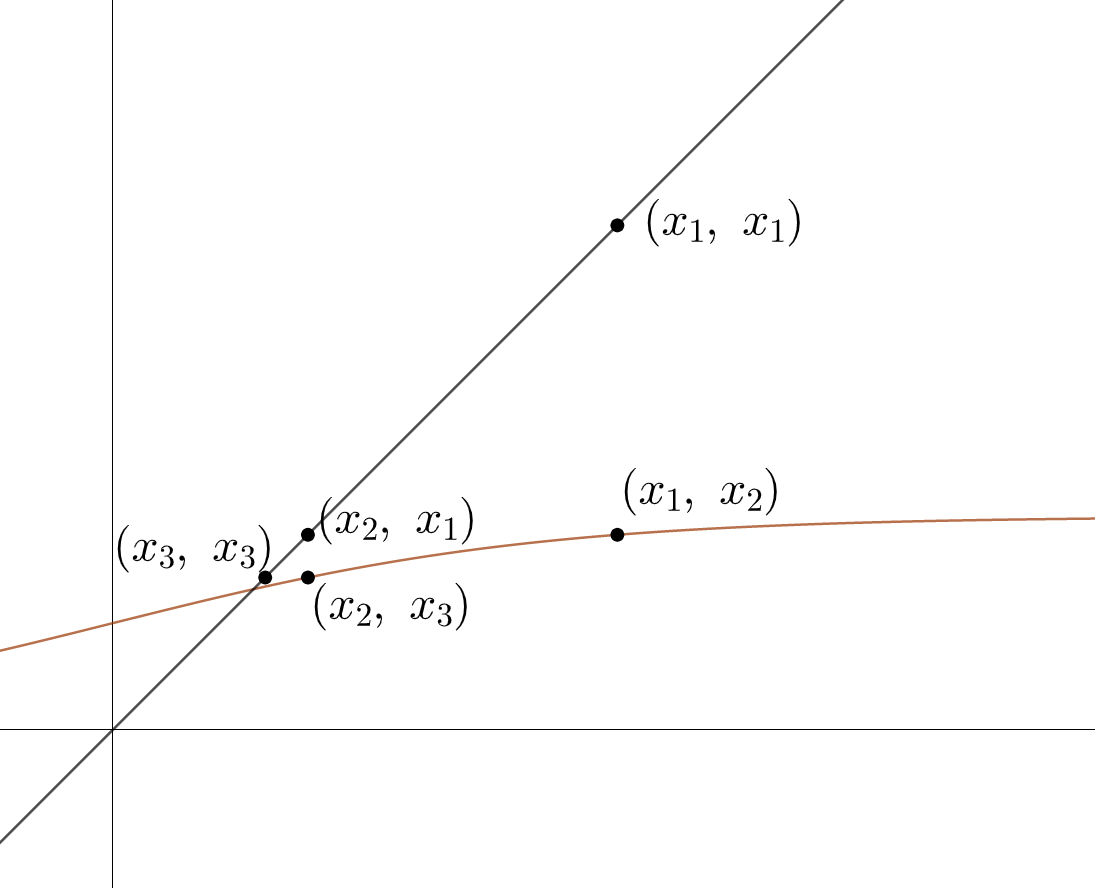
\includegraphics[width=\textwidth]{5_22.png}
			\end{proof}
		\end{spacing}
\end{document}